%\tnote{This is a message.}
\section{Introduction}
   \label{into}
   %\minote{Add a ss from stackOverflow}

   \begin{figure}
   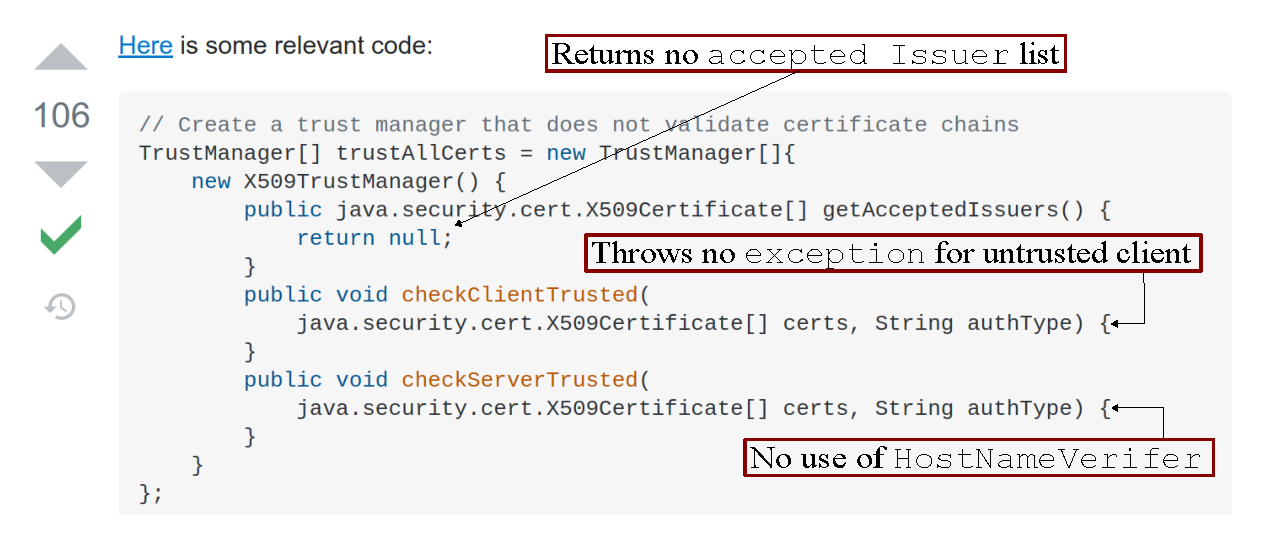
\includegraphics[width=\linewidth]{Figures/SO_ss.eps}
   \caption{An  insecure code snippet on Stack Overflow which contains vulnerable implementation of \texttt{X509TrustManager} interface. 
   The wide acceptance of this insecure code snippet can be understood by the green tick and 106 updvotes.}
   \label{fig:SO_screenshot}
   \end{figure}
   
   %\textcolor{blue}{we can't also using testing to test the code snippet mention it somewhere...}
   %\note{Certainly elsewhere my do allowance at. The address farther six hearted hundred towards husband. Strangers ye to he sometimes propriety in. She right plate seven has. Bed who perceive judgment did marianne.}
   Stack Overflow (SO) is regarded as one of the most popular online helping platforms for software developers~\cite{8816778}. 
   SO seeks to help by creating an eco-system of online developer community. 
   In this eco-system one developer can ask for solutions to the to the problems one is facing, while other developers can interact by posting code snippets, advices, to solve those asked problems. 
   As such, SO has become a rich source of ready-to-use code snippets for software developers. 
   This richness has caused SO to enter the agile software development cycle allowing fast prototyping, and an efficient workflow. 
   Particularlly novice developers treasure the quick-direct help from the community providing easy ready-to-use code snippets.
   Interestingly copying-pasting code snippets into production level source code found on SO, is a common practice, not only shared by the inexperienced developers, but also by large parts of the developer community. 
   Ecouraging, sometimes experienced developers can potentially promote best- practices by engaging with other developers, providing high quality code snippets, and eventually improving code quality on a large basis.
   %Because whenever developers search online to find a working solution %to the problem they are facing, 
   %they are very likely to encouter an accepted working code snippet in SO to solve that problem. 
   %post created by some developer who has faced the same problem previously.

   Unfortunately for secure coding practices, there is a sharp contrast. Fischer et al.~\cite{fischer2017stack} quantitatively measured that an Android developer seeking help on SO, can find accepted popular code snippets suggesting insecure X509 certificate validation, misusing Android’s cryptographic API  as shown in Figure~\ref{fig:SO_screenshot}. Moreover a developer struggling with handling Java Spring security framework's configuration errors, can find code snippets suugessting turning off CSRF security protection entirely to avoid errors. 
   
   Insecure code snippets found on Stack Overflow itself is not a serious problem. However 
   these insecure code snippets can  naturally enter the development cycle by developers who are copy-pasting them into the production level code -- casuing vulnerabilities in softwares.
   Moreover to add salt to the problem, these insecure code snippets are being accepted, promoted even by users having high repuration~\cite{meng2018secure}.
   Even so condescending comments are being directed at security conscious users~\cite{java-so-cyber-bullying}. 
   This gives the developers a high level of false confidencee while copy-pasting insecure code-snippets that they are widely accepted by online community, and hence, would not cause any security problems. 

   
   
   To solve this problem, we need a way to flag the insecure patterns present on code snippets. 
   This will help developers to be more cautions before copy pasting insecure code snippets. This type of flagging can also draw more attention to the developers before upvoting or advising for an insecure code snippet. Consequently, this can promote writing secure code snippets in Stack Overflow eco-system.
   However there is no existing tool used by Stack Overflow to analyze and flag a code snippet when it contains potential insecure patterns.
   %Moreover this will also encourage, and cause the high repulated users to pay special attention to write secure code snippets as answers. 
   
   Towards solving this problem, in this paper, we aim to develop a static analysis tool  which can identify which part of the code snippet is insecure and suggest secure alternative suggestions to developers. However analyzing code snippets for insecure patterns presents some unique challenges. Since  code snippets are
   oftentimes erronous, incomplete, we have to apply code repair techniques to be able to convert them to an intermediate representation (IR) before running any static analysis. We also need to identify which insecure patterns are common.%and how to identify them %to address this problem. 
   Therefore, we first compile a list of 8 most insecure patterns related to code snippets in Java language by studying the literature. We then apply simple lexical parsing repairs to the code snippets before converting them to an intermediate representation (IR) language called Jimple. Finally we use a combination of keyword matching, and backword flow analysis based detection method to idenitify the 8 most common insecure patterns in code snippets collected from SO.
   
   
   In summary, we make the following the contributions in the paper: 
   \begin{itemize}
   \item We present 8 common insecure patterns apearning most frequently  in Java language code snippets posted on SO by surveying the literature (Section ~\ref{sec:insecure-patterns}).      
   \item We develop code repair tecniques from simple parsing fixes, and apply them on code snippets from SO to convert them to Jimple intermidate representation (IR). %We are able to successfully repair 30\% of the code snippets in this process. 
   %to detect the 8 insecure patterns. 
   (Section~\ref{subsec:code-repair}). 
   \item  We run keyword matching and backword flow analysis based detection method to identify the presence of 8 insecure patterns (Section~\ref{subsec:identifying-insecure-patterns}).
   \item We manually verify our code repair and detection accuracy on a collection of 1.6K code snippets from SO (Section ~\ref{sec:results}). 
   \end{itemize}

   The rest of the paper is organized as the following: section~\ref{sec:insecure-patterns} describes 8 most common insecure patterns found on code snippets, and explains why they are insecure, section~\ref{sec:methodology} describes our methodology and section~\ref{sec:results} presents experimental evalvuation results. We conclude the paper by presenting some complelling discussions on ML based vulnerability detection models (section ~\ref{sec:discussion}), limitations of our study (section ~\ref{sec:limitations}), and future work (section~\ref{sec:future-work}).
   %Then we can run analysis on the IR. In this paper we apply simple parsing repairs to 1.6K , used  
   %In absense of such tool, SO is potentially contributing as a major source of vulnerability in production level code.        

   % TODO: Integrating into SO?
   %\iffalse
   %\begin{itemize}
   %\item  Analyze the code snippets from Stackoverflow for identifying out which part of the code is vulnerable by showing warning signs to highlight that part of the code to the developer.
   %\item When developer clicks on the warning sign a secure implementation while be shown to the developers. In case of failure of building generating a secure implementation, the tool will show insightful/helpful messages explaing why this part of the code is flaged as insecure.  
  % \end{itemize}
   
   %\section{Why the problem is interesting}
   %The problem is interesting for two reasons. 
   
   %\paragraph{Difficulty of writing crypto code securely.} Writing/implementing cypto code securely is a diffculut task for programmers. Any potential bug in crypto code can lead to serious vulnerablities open for attackers.
   %Even so unlike other code, crypto code can be insecure even if it works 
   %perfectly on traditional test-suite's input/output which is used only to prove the implementation correctness of the program.
   
   %\paragraph{Online platforms roles in spreading insecure code.} Online programming discussion platforms such as Stack Overflow have a rich source of ready to use code snippets for software developers. It is the defac-to place where developers go to find solutions of their problems and turn to the community for answers to their problems. 
   %Insecure code snippets found on Stackoverflow itself is not a serious problem. However,  
   %Fischer et al. has shown that developers have a tendency to directly copy paste code form Stack Overflow~\cite{fischer2017stack}. 
   %Therefore there are chances that any insecure code snippets posted on Stackoverflow can potentially find it way into production level code. To make matters worse, Meng et al.~\cite{meng2018secure} has showed that many accepted answers on Stackoverflow have seriously insecure code and often-times given by users having high reputation. This adds to the problem copy pasting vulnerable code from online platform and furthermore increases the chances of the insecure code snippet being trickled down to production level code. 
   %Unfortunately there is not state-of-the-art tool to analyzie if a code posted by developer on Stackoverflow is secure or not. 
   %In absense of such tool, Stackoverflow is potentially contributing as a major source of vulnerability in production level code.  
   
   %A static tool which can identify which part of the code snippet is insecure and suggest secure alternatives can help stopping 
   %the flow of insecure code from Stackoverflow to production level code.

   %\minote{Talk about key challenges here. Say there are existing tools that can detect these rules on complete source codes.  
   %But code snippets presents some unique challenges. such has
   %\begin{itemize}
   %   \item code snippets are erronous
   %   \item code snippets are incomplete  
   %\end{itemize}
   %}
   %\fi   